\documentclass[times]{itmo-student-thesis}

%% Опции пакета:
%% - specification - если есть, генерируется задание, иначе не генерируется
%% - annotation - если есть, генерируется аннотация, иначе не генерируется
%% - times - делает все шрифтом Times New Roman, собирается с помощью xelatex
%% - languages={...} - устанавливает перечень используемых языков. По умолчанию это {english,russian}.
%%                     Последний из языков определяет текст основного документа.

%% Делает запятую в формулах более интеллектуальной, например:
%% $1,5x$ будет читаться как полтора икса, а не один запятая пять иксов.
%% Однако если написать $1, 5x$, то все будет как прежде.
\usepackage{icomma}

%% Один из пакетов, позволяющий делать таблицы на всю ширину текста.
\usepackage{tabularx}

%% Данные пакеты необязательны к использованию в бакалаврских/магистерских
%% Они нужны для иллюстративных целей
%% Начало
\usepackage{tikz}
\usetikzlibrary{arrows}
\usepackage{filecontents}
%% Конец

%% Указываем файл с библиографией.
\addbibresource{bachelor-thesis.bib}

\begin{document}

\studygroup{M3435}
\title{Предсказание забытых для модификации файлов на основе Git репозитория}
\author{Рыкунов Николай Викторович}{Рыкунов Н.В.}
\supervisor{Сметанников Иван Борисович}{Сметанников И.Б.}{доцент, к.т.н.}{научный сотрудник университета ИТМО}
\publishyear{2020}
%% Дата выдачи задания. Можно не указывать, тогда надо будет заполнить от руки.
\startdate{01}{сентября}{2018}
%% Срок сдачи студентом работы. Можно не указывать, тогда надо будет заполнить от руки.
\finishdate{31}{мая}{2019}
%% Дата защиты. Можно не указывать, тогда надо будет заполнить от руки.
\defencedate{15}{июня}{2019}

\addconsultant{Поваров Н.И.}{ООО "ИнтеллиДжей Лабс"{}, Аналитик}

\secretary{Павлова О.Н.}

%% Эта команда генерирует титульный лист и аннотацию.
\maketitle{Бакалавр}

%% Оглавление
\tableofcontents

%% Макрос для введения. Совместим со старым стилевиком.
\startprefacepage

\section{Актуальность}
В настоящее время не сложно представить себе такую ситуацию. Предположим, у нас есть команда из двух разработчиков (Р1 и Р2). Однажды произошла приведенная ниже цепочка событий:
    \begin{enumerate}
		\item Р1 пишет некоторый код.
		\item Р1 отправляет изменения на сервер.
		\item Р2 скачивает изменения с сервера, в результате у него появляются изменения Р1.
		\item Р2 собирает проект, запускает код, но программа стала работать неправильно.
		\item Р2 пишет письмо Р1, что Р1 написал некорректно работающий код. 
		\item Р1 исследует проблему и замечает, что он забыл изменить конфигурационный файл, связанный с измененным им раннее кодом.
		\item Р1 модифицирует код в конфигурационном файле.
		\item Р1 отправляет изменения на сервер.
		\item Р2 скачивает изменения с сервера, в результате у него появляются новые изменения Р1.
		\item Р2 собирает проект, запускает код. Теперь программа работает корректно.
	\end{enumerate}
Цепочка событий могла бы быть значительно короче, если бы Р1 не забыл модифицировать конфигурационный файл, который было важно изменить при модификации окружающего кода. В идеальном мире нам хотелось бы всегда видеть такую картину:
    \begin{enumerate}
		\item Р1 пишет некоторый код.
		\item Р1 отправляет изменения на сервер.
		\item Р2 скачивает изменения с сервера, в результате у него появляются изменения Р1.
		\item Р2 собирает проект, запускает код. Теперь программа работает корректно.
	\end{enumerate}
Можно помочь разработчику избежать ошибки, напомнив ему о том, что нужно к текущим измененным файлам так же модифицировать связанные с ними файлами. Модель рекомендации может быть построена так, чтобы предлагать такие <<забытые>> файлы.
\section{Новизна}
\section{Цели и задачи работы}
\section{Практическое значение}
\section{Структура работы}
%% Начало содержательной части.
\chapter{Постановка задачи}
\section{Предметная область}
Git является распределенной системой контроля версий. Система контроля версий помогает разработчику сохранить проделанную работу локально или на сервер. Проектная информация хранится в специальной базе данных, которая называется репозиторий. Репозиторий состоит из некоторого множества снимков изменений, которые именуются коммит. Каждый коммит в свою очередь состоит из ссылки на предыдущий коммит (если имеется), мета-информации (сообщение, автор, время коммита), и самих зафиксированных изменений. В среднем разработчик в большом проекте делает несколько коммитов в день. Они фиксируются в репозитории. Проектов, использующих систему контроля версий Git, большое количество. Таким образом, на данный момент накоплена очень большая кодовая база. Её часть является открытой, например, всем известный сайт GitHub на январь 2020 года содержал более чем 28 миллионов открытых репозиториев. Такая кодовая база неявно хранит в себе шаблоны поведения разработчиков, настройки их окружения и другие интересные для анализа данные. Используя этот набор данных, мы можем помочь разработчикам избежать ошибок, приводивших к неконсистентному состоянию репозитория в прошлом.
%% Так помечается начало обзора.
\section{Постановка задачи}
Введем понятие <<репозиторий>> -- это ориентированное дерево, где каждое ребро представляет из себя отношение <<быть родителем>>. Вершину данного графа будем называть <<коммит>>. Коммит содержит в себе свойства: множество файлов $Files \subseteq File^k$ и мета-информацию (время создания, автор, название коммита). $File \in \mathbb{N}$ -- идентификатор файла в репозитории.\\
\subsection{Требования к ML модели}\label{ml-model-req}
Пусть нам даны репозиторий и коммит из него. Файлы из этого коммита обозначим $TargetCommitFiles \subseteq File^k$. Требуется по данным множеству $CommitFiles \subseteq TargetCommitFiles$, мета-информации о коммите и всех потомках коммита возвращать $TargetCommitFiles$.
\subsection{Требования к реализации}
Требуется разработать плагин для платформы IntelliJ, который во время пользовательского коммита будет рекомендовать пользователю модифицировать и добавить в коммит файлы из репозитория. Плагин должен быть основан на модели, требования к которой изложены в \ref{ml-model-req}. В худшем случае время работы плагина должно составлять не более двух секунд на процессоре 2,2 GHz Quad-Core Intel Core i7. В худшем случае, потребление памяти должно быть не более 10 Мегабайт.
\section{Литературный обзор}
Перед началом выполнения выпускной работы, были проанализировано несколько статей на тему дипломной работы и смежные темы. В мировом индексе представлено множество работ, где рассказано о том, как можно использовать исторические данные в процессе разработки программного обеспечения с целью повышения качества этого процесса. Был подход использования кодовой базы для поиска логически связанных модулей, чтобы отследить, какие файлы изменяются вместе \cite{logical-modules}. В статье \cite{source-change} автор разрабатывал систему предсказаний о том, какие изменения внесет разработчик в кодовую базу. Были проанализированы статьи, которые не имеют непосредственного отношения к выпускной работе, но подходы из этих статей использовались при разработке модели предсказаний. Одна из таких статей \cite{project-memory}. В данной статье авторы разработали приложение Hipikat, позволяющие новым участникам быстрее ознакомится с программной системой, с которой им предстоит работать.
\section{Существующие решения}
\section{Структуризация данных}
\subsection{Исходные данные}
Для получения необработанных данных использовалось названое раннее хранилище репозиториев -- GitHub. Было склонировано несколько репозиториев. История этих репозиториев анализировалась с помощью встроенных в Git комманд (например, git log). Система контроля версий Git выдает историю репозитория, начиная от самых новых коммитов к самым старым. Чтобы упросить анализ, мы анализировали историю из конца в начало, это помогат отслеживать удаление и переименование файлов.
\subsection{Тренировочный датасет}
Когда история репозитория получена, следующий вопрос -- как определить, какие файлы следует рекомендовать для каждого коммита в истории.
\subsubsection{Формат датасета}
Опишем, как выглядит набор данных. Датасет состоит из строк, где любая отдельная строка содержит несколько частей:
    \begin{itemize}
		\item Информация о коммите: автор коммита, время коммита, файлы в нем и т.д.
		\item Файл из репозитория.
		\item Единица, если файл должен быть предсказан, иначе -- ноль.
	\end{itemize}
\subsubsection{Лемма о полном коммите}
Сделаем такое предположение: большинство коммитов в любом репозитории уже содержат полный набор файлов. Учитывая, что коммитов много, коммиты с неполным набором файлов не повлияют на качество рекомендаций.
\subsubsection{Цель}
Если коммит, взятый из репозитория, имеет полный набор файлов, то при удалении файла из этого коммита набор будет неполным. Поэтому цель строится следующим образом: для каждого коммита размера $N$ каждое из его подмножеств размера $N - 1$ берется в качестве первой части, а оставшийся файл считается правильным выходным сигналом -- второй частью строчки датасета. В то же время, система не должна ничего рекомендовать для оригинального коммита, поэтому мы добавляем в датасет некоторое количество строк, где первая часть является текущим коммитом, а вторая часть содержит <<связанный>> файл не из текущего коммита. У такой строчки цель будет равно нулю. <<Связанный>> файл -- это файл, который был в одном и том же коммите с любым из файлов из текущего коммита хотя бы один раз.
\subsection{Тестовый датасет}
Тестовый набор данных имеет тот же формат, что и обучающий набор данных. Самое главное -- никогда не проверять качество системы на данных, которые использовались для обучения этой системы. Поэтому мы проверяем каждый репозиторий на $k$ последних коммитах и обучаем его на остальной истории. Это также имеет и практическое значение -- наша система всегда будет обучаться на данных, полученных в прошлом, значит нам нужно хорошо уметь делать рекомендации в будущем.
\section{Решения}
\subsection{Оценка качества}
Главная цель нашей системы -- рекомендовать полный набор файлов по данному коммиту. Следует отметить, что когда разработчик использует нашу систему, важно не давать неверные рекомендации. Если система не уверена в конкретной рекомендации, то лучше молчать, чем нарушать рабочий процесс разработчика. Исходя из этого предположения, система должна попытаться свести к минимуму количество ложных срабатываний и максимально увеличить количество истинных положительных результатов. Мы должны подумать о том, насколько хороши рекомендации нашей модели со стороны пользователя. Обучающие и тестовые наборы данных были созданы для репозитория IntelliJ IDEA Community. Система рекомендаций по файлам была протестирована на последних 5000 коммитах и обучена на остальных коммитах.
\subsection{Базовый показатель}
Простейшим базовым показателем для нашей системы является получение <<связанных>> файлов, для каждого файла этого набора подсчитайте количество коммитов, в которых содержался этот файл, и порекомендуйте 5 файлов с наибольшим числом.
\subsection{Байесовская оценка}
Следующей попыткой решения поставленной задачи было создание модели баесовской оценки, используя формулу для голосований:
    $$W = v\frac{R}{m + v} + m\frac{C}{m + v},$$
$W$ -- оценка файла, \\
$v$ -- число голосов за то, чтобы предсказать файл, \\
$m$ -- минимальное число голосов за файл $= 3.2$, \\
$R$ -- средняя оценка для файла за предыдущие голосования, \\
${C}$ -- средняя оценка для всех файлов $= 0.25$. \\
Для каждого файла из текущего коммита 20 последних коммитов, содержащих этот файл, извлекаются из истории. После этого каждый из этих извлеченных коммитов голосует за файлы, содержащиеся в нем (исключая файлы от текущего коммита). Величина голоса рассчитывается по формуле: $\min(1.0, \frac{{commit\_size}}{{size}})$\\
$commits\_size$ --  максимальное число файлов в голосующем коммите, чтобы получить максимальную величину голоса $= 8.0$,\\
$size$ -- число файлов в голосующем коммите\\
Результаты из разных файлов складываются. Файл будет рекомендован, если его оценка выше чем порог $= 0,55$.
\section{Планы на будущее}
Наша система считается успешной, когда она предлагает разработчикам некоторые файлы, и они изменяют коммит, добавляя эти файлы более чем в 90\% случаев. Так что есть куда совершенствоваться.

\section{Сбор статистики}
Для того, чтобы понимать, насколько хорошо работает наша решающая функция у пользователей в реальных условиях, а не на искусственно созданном наборе данных, было решено использовать сбор статистики. Также, с помощью пользовательских логов мы сможем понять, что нужно изменить в нашей модели, чтобы число благоприятных исходов увеличилось. Для этого мы запишем факторы для пар файлов и будем использовать их для дальнейшего обучения. Не стоит забывать о том, что очень важно, насколько пользователю подходить интерфейс плагина, используя статистику мы сможем понять реакцию пользователей на наши сообщения. Для этого мы подсчитаем процент случаев, когда пользователь смотрел на предложенные файлы, и когда проигнорировал наше рекомендацию. Всего было сделано две реализации сбора пользовательской статистики. В начале статистика собиралась с использованием серверов JetStat, затем был совершен переход на более современный, встроенный в IntelliJ платформу сервис -- Feature Usage Statistics (FUS).
\subsection{С использованием серверов JetStat}
Первая итерация сбора пользовательских логов использовала сервера внутреннего сервиса сбора и анализа статистики JetStat. Общение с JetStat серверами происходит по протоколу HTTP. Статистика пользователя для JetStat представляется в виде множества строк отчета, их формат будет изложен в секции \ref{report-line}. Отправлять пользовательские логи можно как в сжатом, так и в текстовом виде (для этого используются разные url).
\subsubsection{Модель пользовательских логов}
Пользовательские логи в JetStat представляют из себя конечный автомат. Состояние автомата -- это данные описывающие состояние системы. А переход~-- это пользовательское действие.
\subsubsection{Строка отчета плагина}\label{report-line}
Каждая строка отчета, отправляемого в JetStat, представляет из себя части соединенные символом табуляции:
    \begin{itemize}[label={\textbullet}]
        \item $timestamp$ -- время, когда произошло пользовательское действие.
        \item $recorderId$ -- идентификатор отправителя статистики.
        \item $recoderVersion$ -- версия отправителя статистики.
        \item $userId$ -- идентификатор пользователя (создается при установке IDE).
        \item $sessionId$ -- идентификатор сессии (создается при открытии IDE).
        \item $bucket$ -- идентификатор группы (используется для A/B экспериментов).
        \item $actionType$ -- идентификатор действия пользователя.
        \item $actionJson$ -- информация о состоянии, в которое перешел пользователь.
    \end{itemize}

Рассмотрим конкретнее, какие типы действий пользователя отправлялись плагином:
    \begin{itemize}[label={\textbullet}]
        \item $COMMIT\_CLICKED$ -- нажатие кнопки $Commit$ в $Commit Dialog$.
        \item $CANCEL$ - нажатие кнопки $Cancel$
        \item $COMMIT$ - нажатие кнопки $Commit Anyway$
    \end{itemize}

В информации о состоянии содержался $json$ в котором было несколько полей:
    \begin{itemize}[label={\textbullet}]
        \item $REPOSITORY$ -- уникальный для пользователя идентификатор репозитория.
        \item $FILES$ -- уникальные для репозитория идентификаторы файлов в коммите.
        \item $TIME$ -- время, затраченное на подсчет рекомендации.
        \item $PREDICTION$ -- уникальные для репозитория идентификаторы файлов, рекомендованные для модификации и добавления в коммит.
        \item $FACTORS$ -- факторы посчитанные для каждого рекомендованного файла.
    \end{itemize}
Идентификаторы репозитория, файлов и коммитов создает IntelliJ платформа. По данным идентификаторам нельзя идентифицировать пользователя. Таким образом, никакой приватной информации не отправляется. К тому же, при первом запуске IDE с плагином пользователю показывается нотификация о том, что плагин отправляет полностью анонимные данные для улучшения качества решающей функции.
\subsubsection{Реализация записи и отправки пользовательских логов}
\begin{figure}[!h]
\caption{Схема записи и отправки пользовательских логов}\label{jet-stat-logs}
\centering
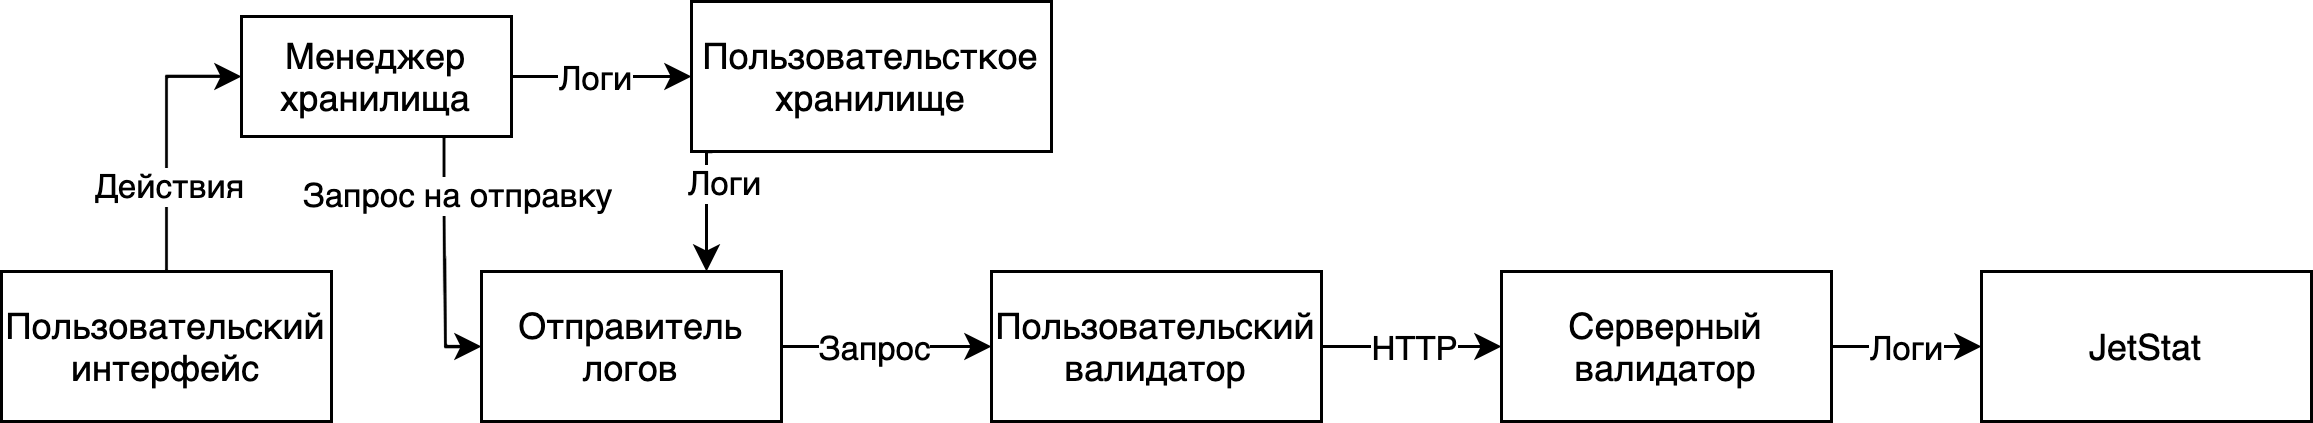
\includegraphics[scale=0.2]{JetStat.png}
\end{figure}
Реализация записи и отправки пользовательских логов показана на рисунке \ref{jet-stat-logs}. Принцип работы является достаточно популярным. При совершении пользователем какого-то действия над интерфейсом, это действие отправляется к менеджеру хранилища, который создает правильные строки отчета и сохраняет их в локальное хранилище. После этого менеджер хранилища отправляет запрос отправителю логов, чтобы сервис отправил накопившиеся данные на сервер. Если данных в локальном хранилище достаточно, то из них отправитель логов собирает HTTP запрос на сервер. Затем идет переход к одной из самых важных частей реализации -- валидаторы. Перед тем, как отправлять данные на сервер, очень важно понять, не нарушена ли их консистентность (например, пользователю была показана рекомендация, но он ничего с ней не сделал). Для проверки консистентности данных был создан валидатор, который присутствует, как на стороне клиента, так и на стороне сервера. Только после того, как HTTP запрос прошел валидацию на клиентской стороне, он отправляется на сервер JetStat, где расположен серверный валидатор. Если пришедшие данные консистентны, то они сохраняются на сервер и ждут дальнейшей обработки.
\subsection{С использованием Feature Usage Statistics}
Следующая итерация сбора статистики плагина использовала сервис Feature Usage Statistics (FUS). FUS встроен в IntelliJ платформу.
\subsubsection{Модель пользовательских логов}
Пользовательские логи сервиса FUS представляют из себя набор событий системы. Часто, но не всегда, эти события порождаются действиями пользователя.
\subsubsection{Реализация отправки пользовательских логов}
Отправка пользовательских логов с помощью сервиса FUS является более простой в сравнении с отправкой статистики на сервера JetStat. Feature Usage Statistics сам занимается хранением, валидацией, отправкой данных. Нашему приложению достаточно собрать $FeatureUsageData$ объект и передать его в FUS.
\printmainbibliography

\end{document}